\documentclass[tikz,border=10pt]{standalone}
\usepackage{amsmath}
\begin{document}
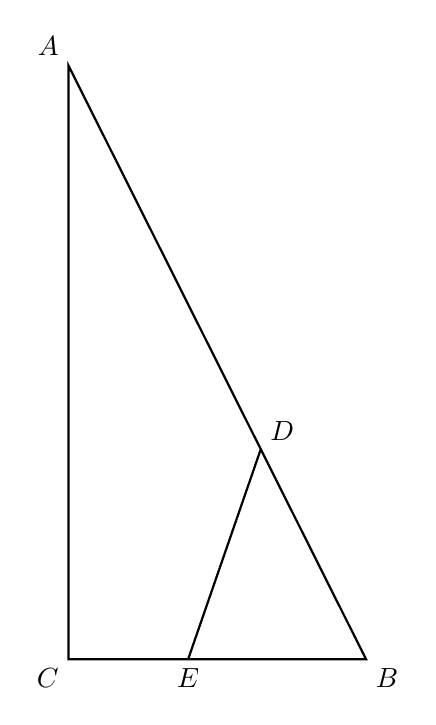
\begin{tikzpicture}[scale=1]
  \coordinate (C) at (0,0);
  \coordinate (B) at (3.78,0);
  \coordinate (A) at (0,7.54);
  \coordinate (D) at (2.44,2.66);
  \coordinate (E) at (1.52,0);

  \draw[thick] (A) -- (C) -- (B) -- cycle;
  \draw[thick] (D) -- (E);

  \node[above left] at (A) {$A$};
  \node[above right] at (D) {$D$};
  \node[below left] at (C) {$C$};
  \node[below] at (E) {$E$};
  \node[below right] at (B) {$B$};
\end{tikzpicture}
\end{document}
